\documentclass[12pt, titlepage]{article}


% Author's up-front packages
\usepackage[T1]{fontenc}
\usepackage[utf8]{inputenc}
\usepackage{longtable}

%Packages from template
\usepackage{amsmath, mathtools}
%\usepackage[round]{natbib}
\usepackage{amsfonts}
\usepackage{amssymb}
\usepackage{graphicx}
\usepackage{colortbl}
\usepackage{xr-hyper}
\usepackage{hyperref}
\usepackage{xfrac}
\usepackage{tabularx}
\usepackage{float}
\usepackage{siunitx}
\usepackage{booktabs}
\usepackage{multirow}
\usepackage[section]{placeins}
\usepackage{caption}
\usepackage{fullpage}

% Author's packages

\usepackage{cite}
\usepackage{indentfirst}
\usepackage{csquotes}
\usepackage{cleveref}

\hypersetup{
%bookmarks=true,     % show bookmarks bar?
colorlinks=true,       % false: boxed links; true: colored links
linkcolor=red,          % color of internal links (change box color with linkbordercolor)
citecolor=blue,      % color of links to bibliography
filecolor=magenta,  % color of file links
urlcolor=cyan          % color of external links
}

\usepackage{array}

%% Comments

\usepackage{color}

\newif\ifcomments\commentstrue

\ifcomments
\newcommand{\authornote}[3]{\textcolor{#1}{[#3 ---#2]}}
\newcommand{\todo}[1]{\textcolor{red}{[TODO: #1]}}
\else
\newcommand{\authornote}[3]{}
\newcommand{\todo}[1]{}
\fi

\newcommand{\wss}[1]{\authornote{blue}{SS}{#1}}
\newcommand{\an}[1]{\authornote{magenta}{Author}{#1}}


\newcommand{\progname}{STEM Moir{\'e} GPA}
\externaldocument[SRS:]{../SRS/SRS}
\externaldocument[TP:]{../TestPlan/TestPlan}
\externaldocument[MG:]{../Design/MG/MG}
\externaldocument[MIS:]{../Design/MIS/MIS}
\externaldocument[TP:]{../TestPlan/TestPlan}

%Set the custom referencing syste
	% Module
\newtheorem{M}{M}
\crefname{M}{M}{Ms}
	% Module Interface Specification
\newtheorem{MIS}{MIS}
\crefname{MIS}{MIS}{MISs}
	% Requirements
\newtheorem{R}{R}
\crefname{R}{R}{Rs}
	% Instance Model
\newtheorem{IM}{IM}
\crefname{IM}{IM}{IMs}
	% Test
\newtheorem{Test}{Test}
\crefname{Test}{Test}{Tests}
	% Theoretical Model
\newtheorem{T}{T}
\crefname{T}{T}{Ts}
	% Data Definition
\newtheorem{DD}{DD}
\crefname{DD}{DD}{DDs}
	% Test Report
\newtheorem{TestRep}{TestRep}
\crefname{TestRep}{TestRep}{TestReps}

\begin{document}

\title{User Guide: STEM Moir{\'e} GPA} 
\author{Alexandre Pofelski \\
		macid: pofelska \\
		github: slimpotatoes}
\date{\today}
	
\maketitle

\pagenumbering{roman}

\section{Revision History}

\begin{tabularx}{\textwidth}{p{3cm}p{2cm}X}
\toprule {\bf Date} & {\bf Version} & {\bf Notes}\\
\midrule
19/12/2017 & 1.0 & First quick version\\
\bottomrule
\end{tabularx}

~\newpage

\section{Symbols, Abbreviations and Acronyms}

The same Symbols, Abbreviations and Acronyms as in the SRS, the TestPlan, the 
MG and the MIS documents (available in 
\href{https://github.com/slimpotatoes/STEM_Moire_GPA}{\progname{}} repository) 
are used in the User Guide document. 

\newpage

\tableofcontents

\listoftables %if appropriate

\listoffigures %if appropriate

\newpage

\pagenumbering{arabic}

\section{Introduction}

The aim of the document is to provide to the end user of \progname{} some guidance to operate the software properly. The software is still under development therefore, it is very likely to find some bugs when executing the code. Considerable updates are planned to be performed nevertheless, the general use of the software should not be drastically modified. The document proposes a walkthrough of each step of \progname{} processing using the files available in the \enquote{Examples} folder.

\section{Before executing \progname{}}

The user responsibilities are described in the SRS document, nevertheless it is worth mentioning that a minimum of two files are required to execute \progname{} which are:
\begin{itemize}
\item a calibrated STEM Moir{\'e} hologram (only .dm3 files are working for the moment)
\item a calibrated Reference image (only .dm3 files are working for the moment)
\end{itemize}

A STEM Moir{\'e} hologram is a STEM electron micrograph in which at least one crystal periodicity is under sampled. A classic STEM electron micrograph can still be used with \progname{} however, the software becomes a classic Geometrical Phase Analysis software.\medskip

A Reference image is an experimental STEM electron micrograph or a simulated image in which none of the crystal periodicities are under sampled. It is required, for the reference image, to represent precisely the same crystal lattice of the sample from which the STEM Moir{\'e} hologram has been acquired and preferably at its unstrained state.\medskip

One STEM Moir{\'e} hologram with its associated Reference image are present in the \enquote{Examples} folder. Those two files are going to be used in the following steps.

\section{Starting \progname{}}

After downloading the source files and checking that the requirement from the dependencies are met, the main.py file can be executed and two windows should appear.Do not close these windows since there is no way of reopening them without starting the software again. The first window (\cref{fig:SMG_Flow}) corresponds to \progname{} flow with all the different buttons that represent the different steps of execution which are (details of each step will be describe later in the document):
\begin{itemize}
\item \enquote{Input}: Load the two required files
\item \enquote{SMHSim}: Simulate the STEM Moir{\'e} hologram from the Reference image to get the (n,m) shift for the conversion
\item \enquote{GPA}: Execute the GPA algorithm to output the variation of the Moir{\'e} wave vector.
\item \enquote{Ref}: Define an area of the STEM Moir{\'e} hologram as the unstrained reference
\item \enquote{Convert}: Convert the Moir{\'e} wave vectors into their respective crystalline wave vectors.
\item \enquote{Strain}: Calculate and display the 2D strain tensor from two non collinear crystalline wave vector.
\end{itemize}

\begin{figure}[H]
\centering
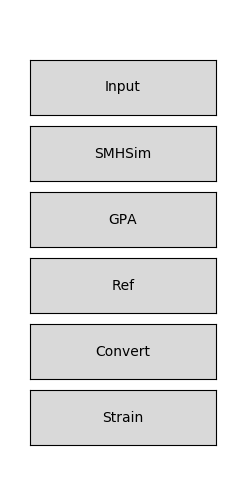
\includegraphics[scale=1]{Figures/SMG_Flow.png}
\caption{\progname{} window flow}
\label{fig:SMG_Flow}
\end{figure}

The second window (\cref{fig:nm_shift}) is composed of entry fields to let the user choose the shift to perform to convert the chosen Moir{\'e} wave vector to its corresponding crystalline wave vector. Only integer numbers are accepted in the entry field.

\begin{figure}[H]
\centering
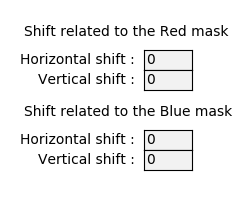
\includegraphics[scale=1]{Figures/(n,m)_shift.png}
\caption{Conversion window}
\label{fig:nm_shift}
\end{figure}

\section{Load files}

To load the required files, select the \enquote{Input} button in \progname{} window flow. A dialog will appear (\cref{fig:load_files}) requesting you to choose first the STEM Moir{\'e} hologram and then the Reference image. An error message should appear if the loading process was not performed properly. At the end of the loading process a new window with the STEM Moir{\'e} hologram and reference image should appear (\cref{fig:SMH_and_ref})

\begin{figure}[H]
\centering
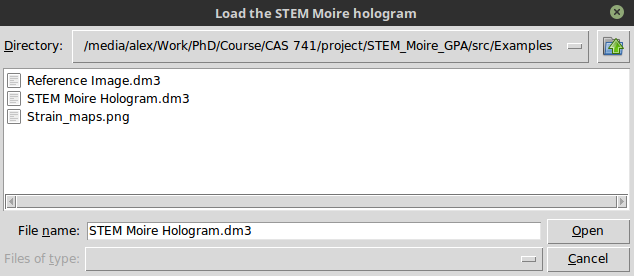
\includegraphics[scale=0.7]{Figures/Load_files.png}
\caption{Load file dialog}
\label{fig:load_files}
\end{figure}

\begin{figure}[H]
\centering
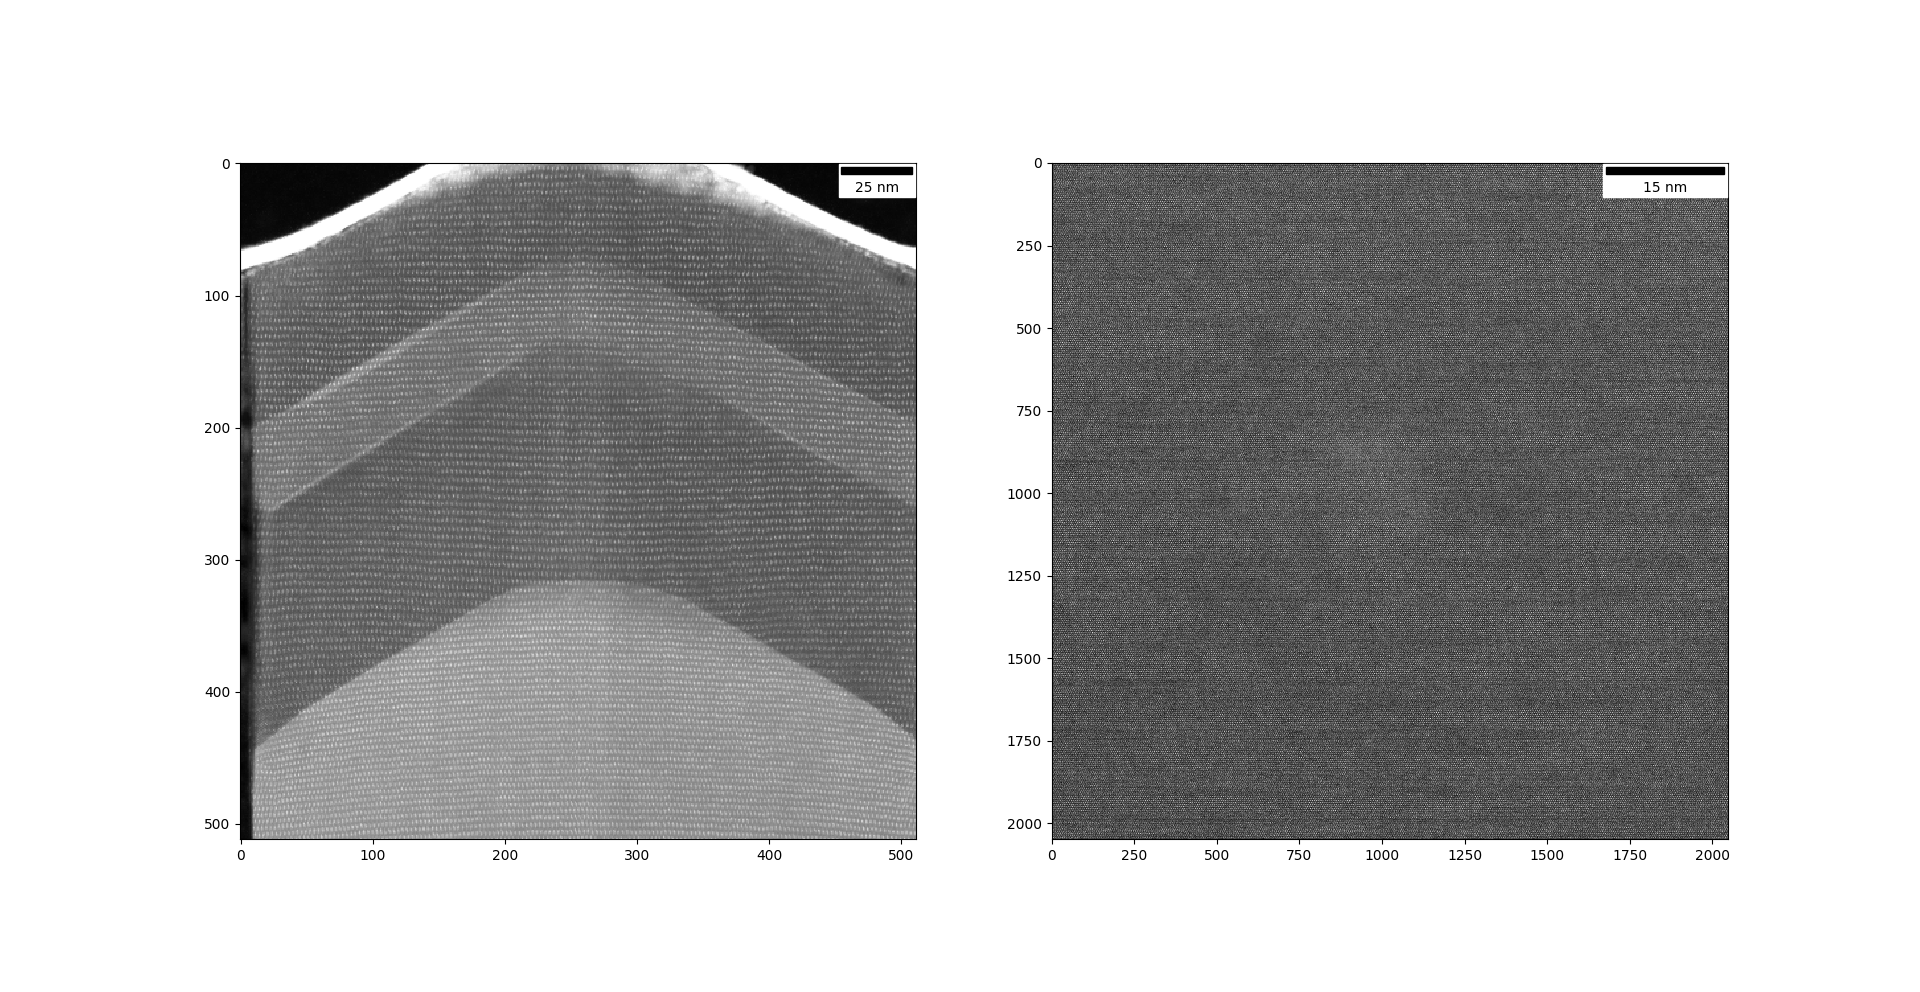
\includegraphics[scale=0.35]{Figures/SMH_and_reference_image.png}
\caption{STEM Moir{\'e} hologram and reference image window}
\label{fig:SMH_and_ref}
\end{figure}

\section{Simulate the STEM Moir{\'e} hologram}

Once the files loaded, select the \enquote{SMHSim} button to launch the simulation process. Please be patient, this step can take some time. At the end of the simulation, three windows will appear:
\begin{itemize}
\item the \enquote{SMH simulation window} \cref{fig:SMH_Simulation}: this is the most important window and should not be closed at any time since it is used in the next steps of \progname{} processing. On the left image is presented the Fourier Transform of the experimental STEM Moir{\'e} hologram with a red and a blue circle (their role will be describe later). On the right image is shown the Fourier transform of the simulated unstrained STEM Moir{\'e} hologram from the reference image. The user should be able to identify some correspondence between the two images (position and arrangement of the reflections). If it is not the case, the reference image is probably inappropriate. 

\begin{figure}[H]
\centering
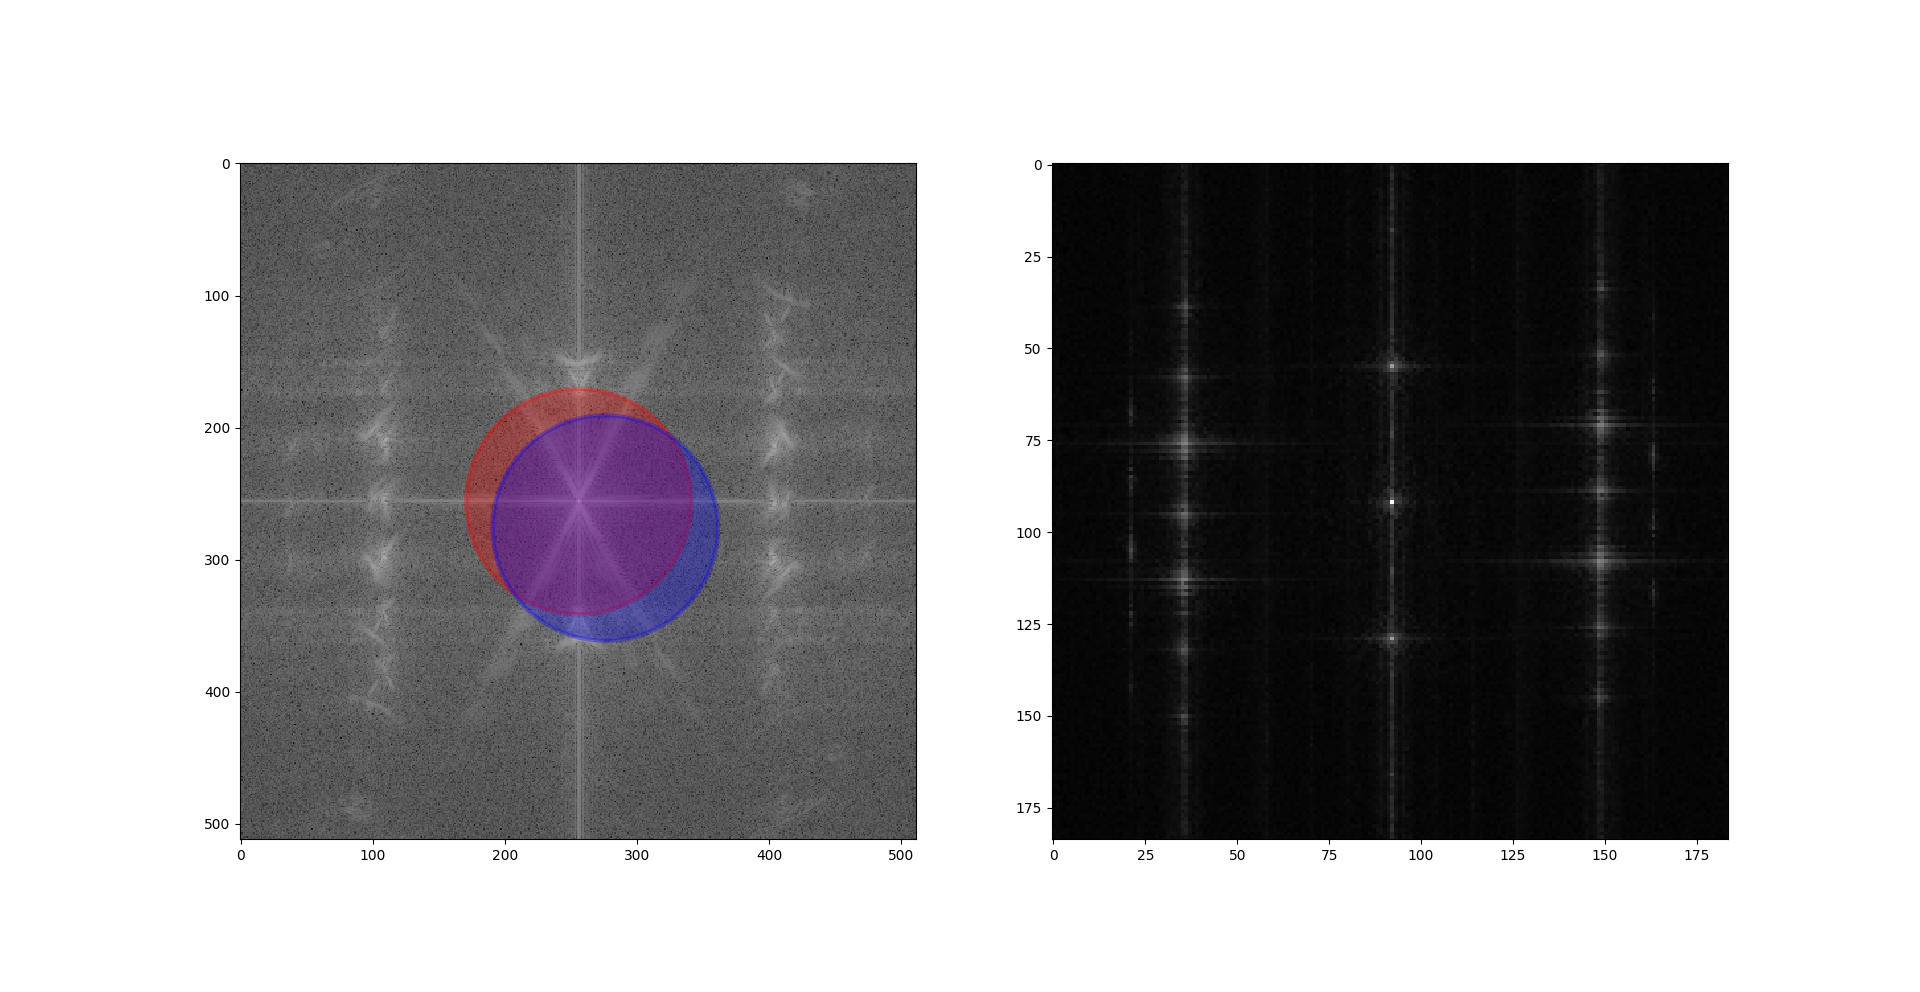
\includegraphics[scale=0.35]{Figures/SMH_Simulation.png}
\caption{STEM Moir{\'e} hologram simulation window}
\label{fig:SMH_Simulation}
\end{figure}

\item the \enquote{SMH Simulated with colors} (\cref{fig:SMH_Simulated_colors}): this window follows the same color code as  \enquote{Ic split into tiles} and represents the Fourier transform of the simulated STEM Moir{\'e} hologram. It is the identical version of the one present in the \enquote{SMH simulation window} but with colors and more noise. The colors are here to help in distinguishing the different reflections.

\begin{figure}[H]
\centering
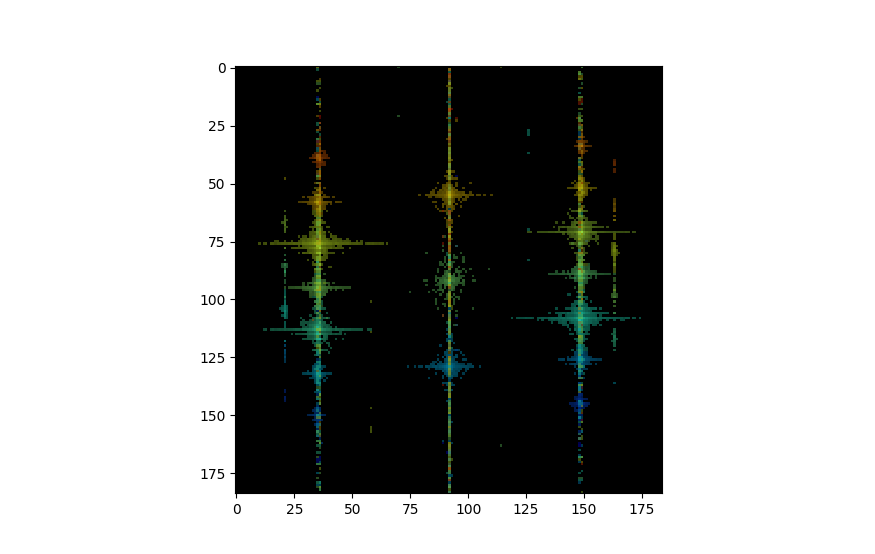
\includegraphics[scale=0.8]{Figures/Simulated_SMH_with_colors.png}
\caption{STEM Moir{\'e} hologram simulated with colors window}
\label{fig:SMH_Simulated_colors}
\end{figure}

\item the \enquote{Ic split in tiles} (\cref{fig:Ic_split_tiles}): this window needs to be read in parallel with \enquote{SMH Simulated with colors} and represents the effect of sampling on the reference image. The separation in tiles with different colors is to make the link between the reflection position in enquote{SMH Simulated with colors} and the tiles they originate.

\begin{figure}[H]
\centering
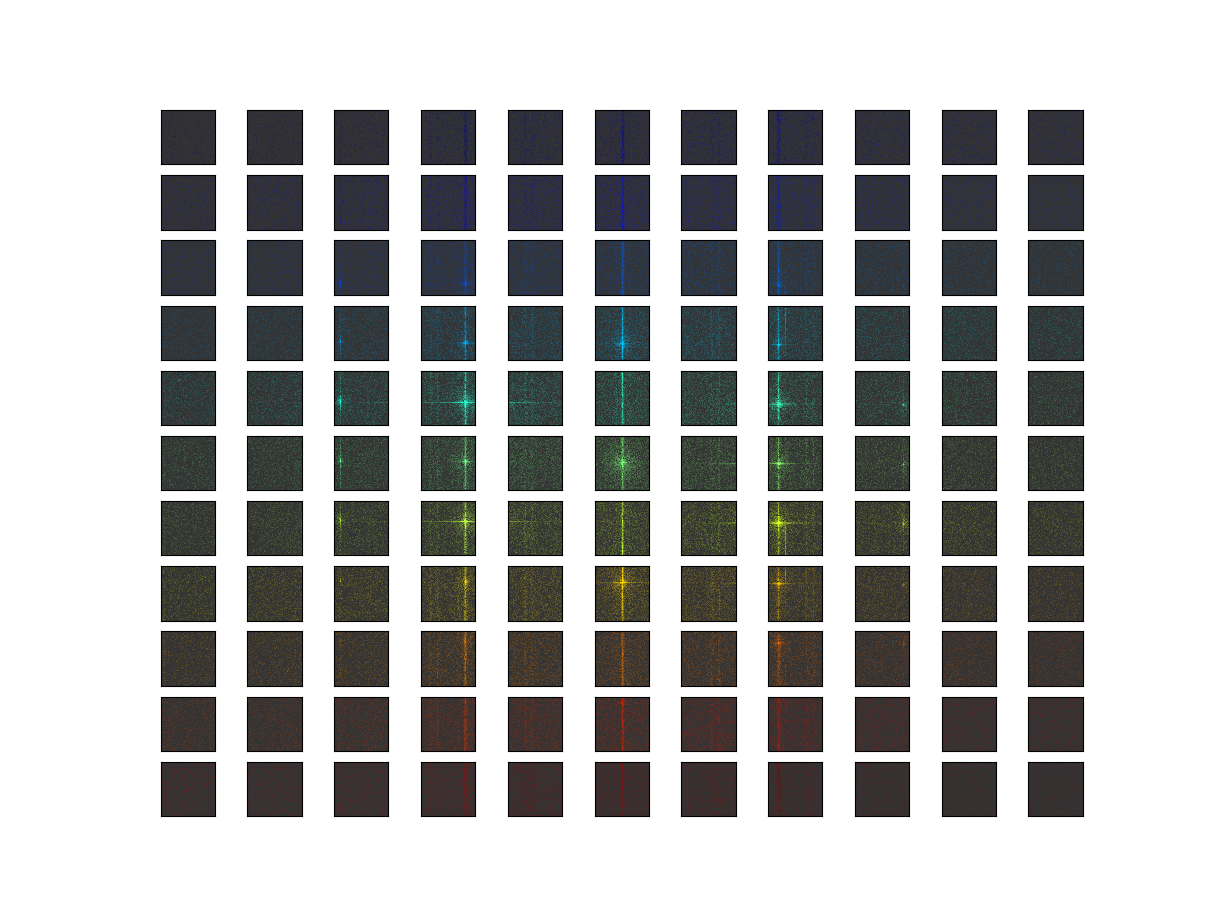
\includegraphics[scale=0.5]{Figures/Ic_split_into_tiles.png}
\caption{Reference image split in tiles window}
\label{fig:Ic_split_tiles}
\end{figure}
\end{itemize}

The goal of the simulation step is to read the necessary shift to convert the Moire wave vector into the crystalline wave vector. \Cref{fig:shift_extraction} is summarizing the sampling process and the shift effect on the tiles (some notion of crystallography is advised to interpret the data). The sampling effect can be imaged by considering the overlap (or the sum) of each individual tile into the central tiles. Taking for example the tile $g_{0002}$ circled in blue in \cref{fig:shift_extraction}, a \enquote{(-2,0) shift} (2 vertical shift down and 0 horizontal shift) brought by the undersampling condition, is adding the contribution from the $g_{0002}$ tile into the central tile. The contribution on the central tile of the $g_{0002}$ tile can be found on the Fourier transform of the simulated STEM Moir{\'e} hologram (right image in \cref{fig:shift_extraction}) by finding the corresponding color. The same methodology can be applied for the $g_{1-100}$ tile circled in green. In this case a \enquote{(0,-2)} shift is generated by the undersampling condition to add the contribution of the $g_{1-100}$ tile in the central tile.

\begin{figure}[H]
\centering
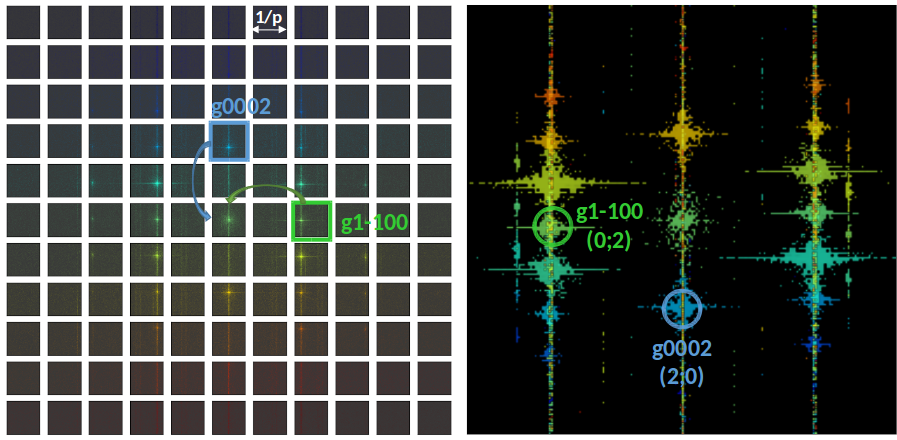
\includegraphics[scale=0.5]{Figures/Read_simulation.png}
\caption{Extract the shift from the simulation data. On the left is shown the reference image split in tiles and on the right is shown the Fourier transform of the simulated STEM Moir{\'e} hologram.}
\label{fig:shift_extraction}
\end{figure}

The two shifts identified and their contribution localized in the Fourier transform of the \textbf{simulated} STEM Moir{\'e} hologram, the correspondence can be done on the Fourier transform of the \textbf{experimental} STEM Moir{\'e} hologram. An example is shown in \cref{fig:shift_extraction_2} where corresponding reflections are first identified on the experimental data (by analogy with the simulated one). Then, to compensate the undersampling effect, the opposite shifts compared to the ones earlier identified need to be considered to recover the original signal from the crystal. Therefore, the shift, for the conversion process, for the $g_{0002}$ reflection will be (2,0) (Shift vertical = 2 and shift horizontal = 0) and (0,2) for the $g_{1-100}$ reflection (Shift vertical = 0 and shift horizontal = 2). These sets of shifts are the ones that are going to be used to fill the entry fields of the conversion window (\cref{fig:nm_shift}) before executing the conversion process.

\begin{figure}[H]
\centering
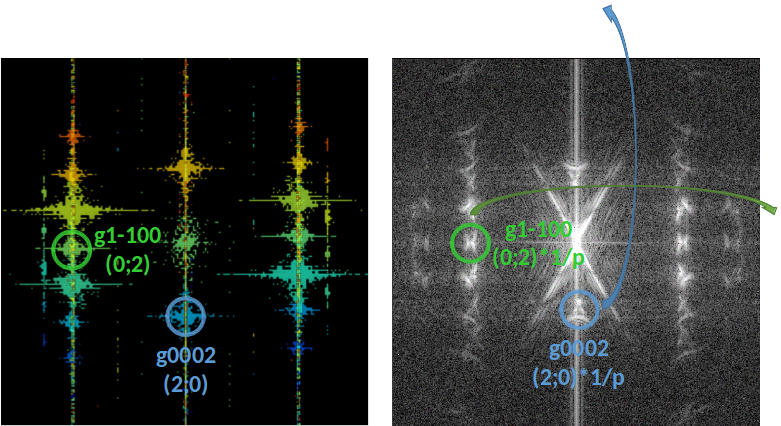
\includegraphics[scale=0.6]{Figures/Read_simulation_2.png}
\caption{On the left is shown the Fourier transform of the simulated STEM Moir{\'e} hologram and on the right the Fourier transform of the experimental STEM Moir{\'e} hologram.}
\label{fig:shift_extraction_2}
\end{figure}

Once the shift determined, the \enquote{Ic split in tiles} and the \enquote{SMH Simulation with colors} windows can be closed. Those won't be reused in the following steps.

\section{GPA}

With the GPA algorithm, the user wants to isolate a particular spatial frequency to capture the variation of the wave vector. With the previous step, the user should have identified two non collinear reflections in the Fourier transform of the experimental STEM Moir{\'e} hologram. Those two reflections are the ones that are going to be selected using the red and the blue circle available in the window. The position and the radius of the circles will define the mask that are going used by the GPA module.\medskip

To edit the position and the radius of both circles, the user should press the letter "e" on the keyboard (while having the \enquote{SMH simulation window} \cref{fig:SMH_Simulation} active) to toggle the editing mode of the window. Then, select the circle with the left click to position it on the selected reflection and modify the radius using the right click of the mouse. The position and the radius of the circles have non negligible effects on the performance of the GPA algorithm (resolution and sensitivity). The effects are described in the Test Report document and should be use as recommendations to find the proper conditions. Once the circles are positioned properly (by isolating respectively one isolated feature only), the user should press the letter "d" to lock the properties of the circles and turn off the edit mode. If needed the user can press "e" again to turn on the edit mode. When the modification finished, it is mandatory for the user to turn off the editing mode for the GPA function to be executed.\medskip

\Cref{fig:SMH_Simulation_1} is an example of what a user should get after editing the position and the radius of the circles. It is possible to note that one circle is filled and the other one is unfilled. The difference is to identify the circle that has been selected for the GPA process. The selected mask is the one which is unfilled. 

\begin{figure}[H]
\centering
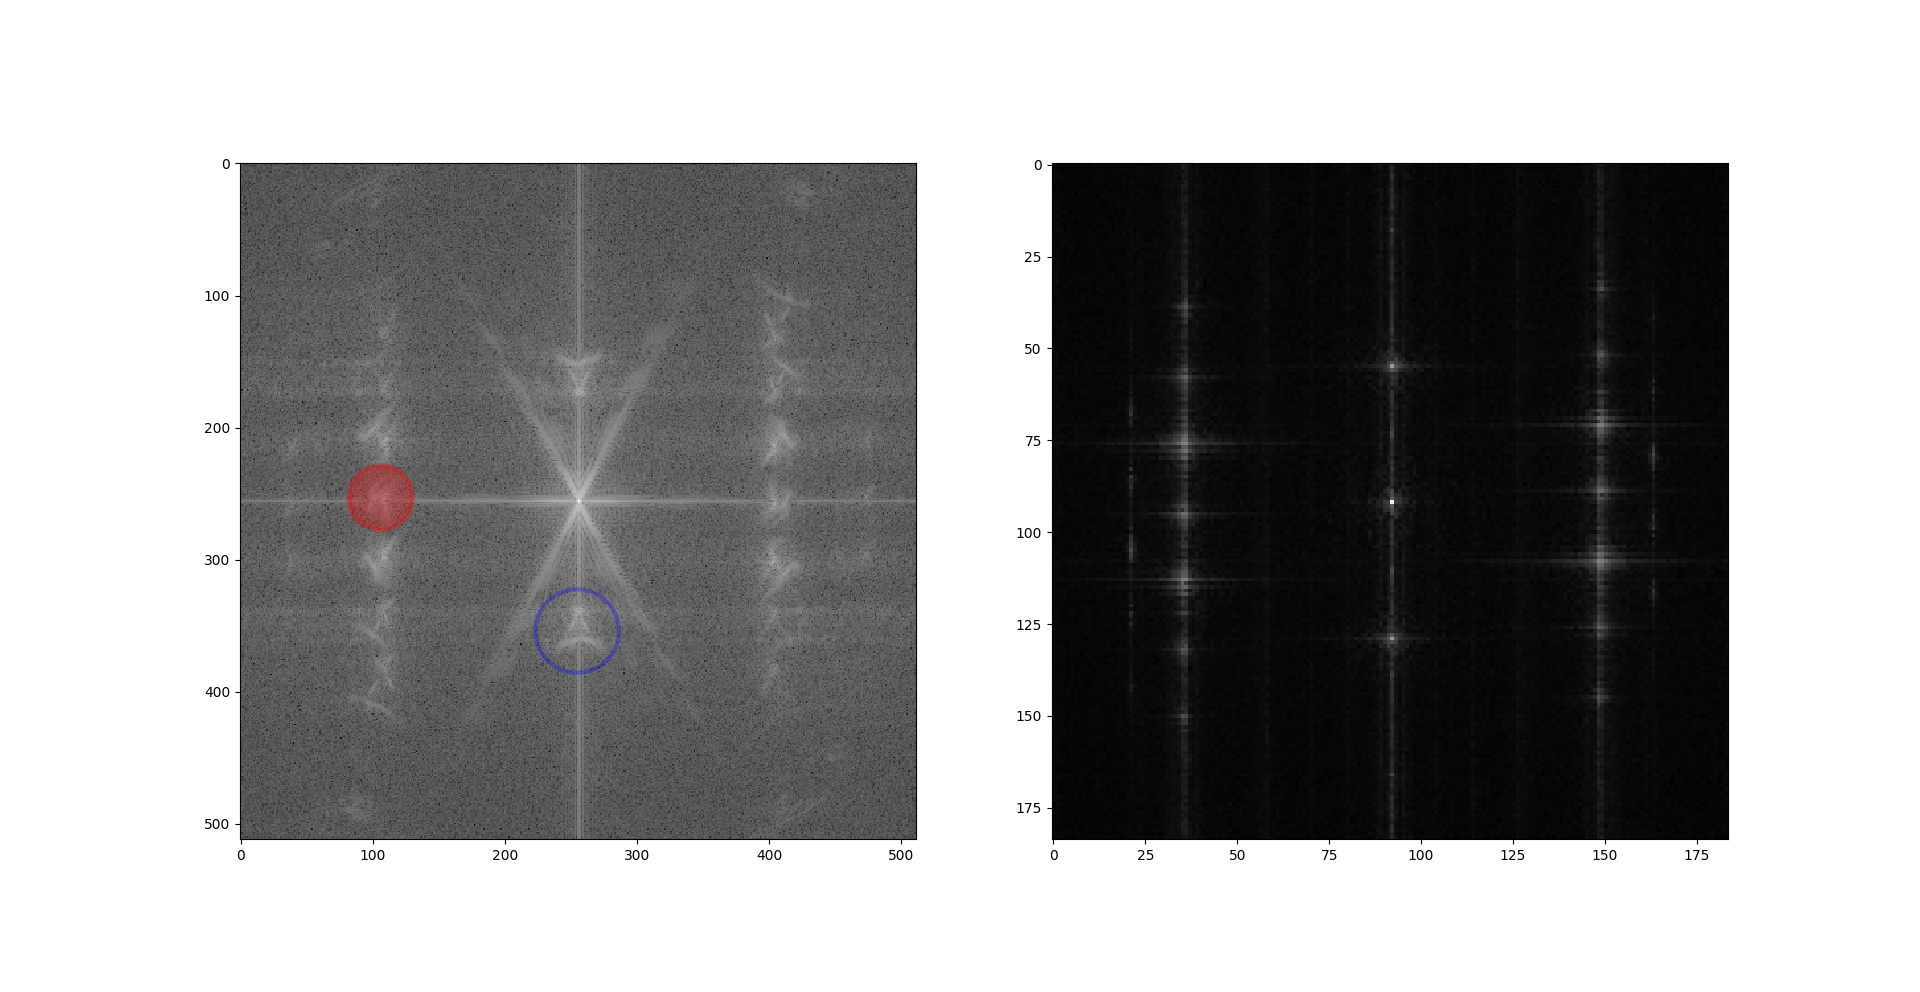
\includegraphics[scale=0.35]{Figures/SMH_Simulation-1.png}
\caption{STEM Moir{\'e} hologram simulation window with the mask positioned}
\label{fig:SMH_Simulation_1}
\end{figure}

\bibliographystyle{ieee}

\bibliography{UserGuide}

\end{document}